\section{GFNT 自訂點陣字型格式}
\label{app:gfnt}

\subsection{設計動機}

FreeGLUT 內建 Bitmap/Stroke 字型不足以涵蓋中文，因此程式使用簡單的 GFNT binary resource。格式採用固定大小的 header 與 glyph entry，載入時可以先檢查檔案範圍，之後再依排序過的 Unicode code point 做 binary search。正文的圖~\ref{fig:gfnt-runtime} 已整理文字繪製的主流程；本附錄再分別說明檔案結構、Loader 檢查與找不到字元時的 fallback。

\subsection{Binary Layout}

格式使用 1-byte packing，並由 C++ 的 static assertion 確認 GfntHeaderV1 為 16 bytes、GfntGlyphV1 為 18 bytes。檔案中的整數欄位一律使用 little-endian。若 Glyph 數量為 $N$，Bitmap Data 的檔案 offset 就是 $16+18N$。圖~\ref{fig:gfnt-layout} 與表~\ref{tab:gfnt-fields} 都依照目前程式中的 struct 欄位與大小整理。

\begin{figure}[H]
    \centering
    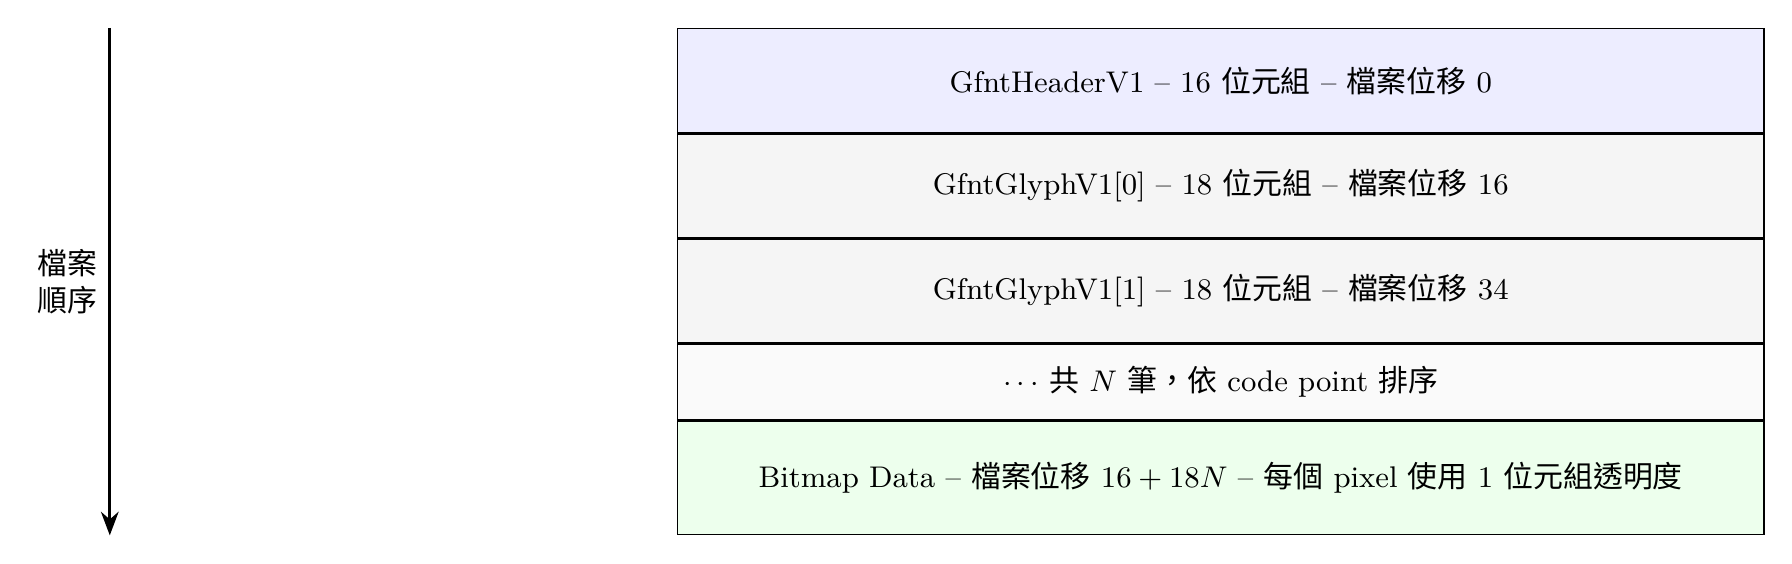
\includegraphics[width=.94\textwidth]{docs/figures/app_b_gfnt-layout.png}
    \caption{GFNT v1 二進位檔案配置}
    \label{fig:gfnt-layout}
\end{figure}

\begin{longtable}{>{\ttfamily}l r r l}
    \caption{GFNT v1 欄位、相對 offset 與大小}\label{tab:gfnt-fields}           \\
    \toprule
    Field        & Offset & Size & Meaning                              \\
    \midrule
    \endfirsthead
    \toprule
    Field        & Offset & Size & Meaning                              \\
    \midrule
    \endhead
    \multicolumn{4}{l}{\normalfont\textbf{GfntHeaderV1 (16 bytes)}}     \\
    magic        & 0      & 4    & ASCII \lstinline|GFNT|               \\
    version      & 4      & 2    & 格式版本，目前為 1                           \\
    pixelSize    & 6      & 2    & nominal pixel size，不可為 0             \\
    ascender     & 8      & 2    & baseline 上方高度，\lstinline|int16_t|    \\
    descender    & 10     & 2    & baseline 下方高度，\lstinline|int16_t|    \\
    glyphCount   & 12     & 4    & glyph table entry 數量                 \\
    \midrule
    \multicolumn{4}{l}{\normalfont\textbf{GfntGlyphV1 (18 bytes each)}} \\
    codepoint    & 0      & 4    & Unicode codepoint                    \\
    width        & 4      & 2    & bitmap 寬度                            \\
    height       & 6      & 2    & bitmap 高度                            \\
    bearingX     & 8      & 2    & pen 到 bitmap 左側的水平位移                 \\
    bearingY     & 10     & 2    & baseline 到 bitmap 頂端的垂直位移            \\
    advanceX     & 12     & 2    & 下一個 pen X 增量                         \\
    bitmapOffset & 14     & 4    & 相對 Bitmap Data 開頭的 byte offset       \\
    \bottomrule
\end{longtable}

\subsection{Loader 與驗證}

Loader 先取得檔案大小，確認至少能容納 16-byte header，再逐欄讀取不同寬度的整數。接著檢查 magic、version、pixel size、ascender、descender，以及 $16+18N$ 是否超出檔案。Bitmap Data 讀完後，程式還會逐一檢查 Glyph：code point 必須按照遞增順序排列，不得超過 U+10FFFF 或落在 surrogate 範圍，而且流程如圖~\ref{fig:gfnt-loader-validation} 所示。

\begin{figure}[H]
    \centering
    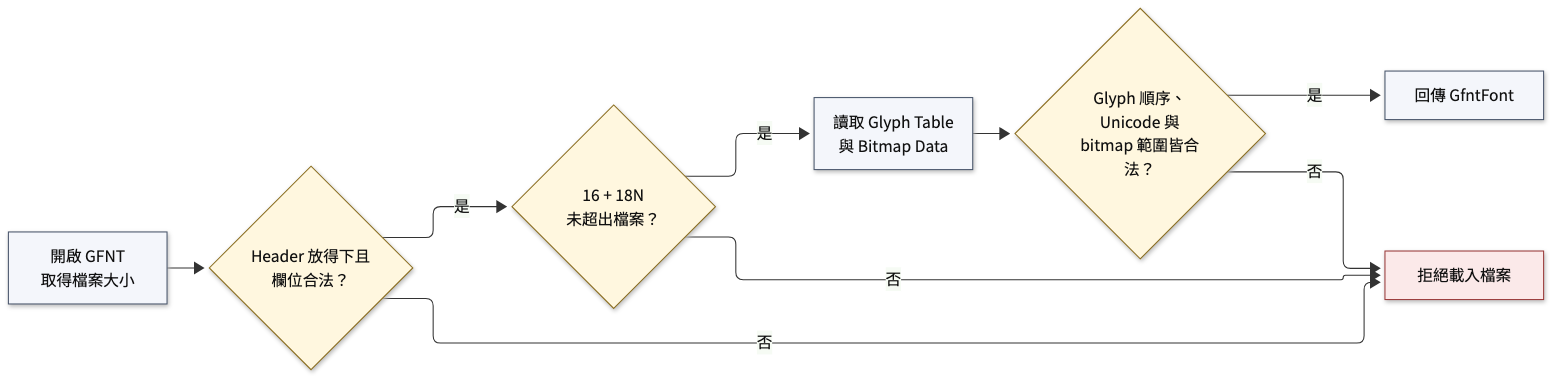
\includegraphics[width=.96\textwidth]{docs/figures/app_b_gfnt-loader-validation.png}
    \caption{GFNT Loader 的讀取與驗證順序}
    \label{fig:gfnt-loader-validation}
\end{figure}

\[
    o + w\times h
    \le \text{Bitmap Data size}.
\]

其中 $o$、$w$、$h$ 分別對應 \lstinline|bitmapOffset|、\lstinline|width| 與 \lstinline|height|。程式實際以減法形式比較，避免加法 overflow。這些檢查都在載入字型時完成，render loop 不需要每畫一個字就重新檢查。

\subsection{UTF-8 Decoder 與 Glyph Lookup}

UTF-8 decoder 會檢查 sequence 長度、continuation bytes、最小合法值、最大 code point 與 surrogate，遇到錯誤時消耗一個 byte 並回傳 U+FFFD。Glyph Table 在載入時已確認順序，因此查找時使用 \lstinline|std::lower_bound|；若找不到原字元，再依序嘗試 U+FFFD 與問號。圖~\ref{fig:gfnt-glyph-lookup} 對應 \lstinline|findGlyphOrFallback()| 的實際查找順序；三次都找不到時，Renderer 以 header 的 pixel size 推進 pen，而不繪製 bitmap。

\begin{figure}[H]
    \centering
    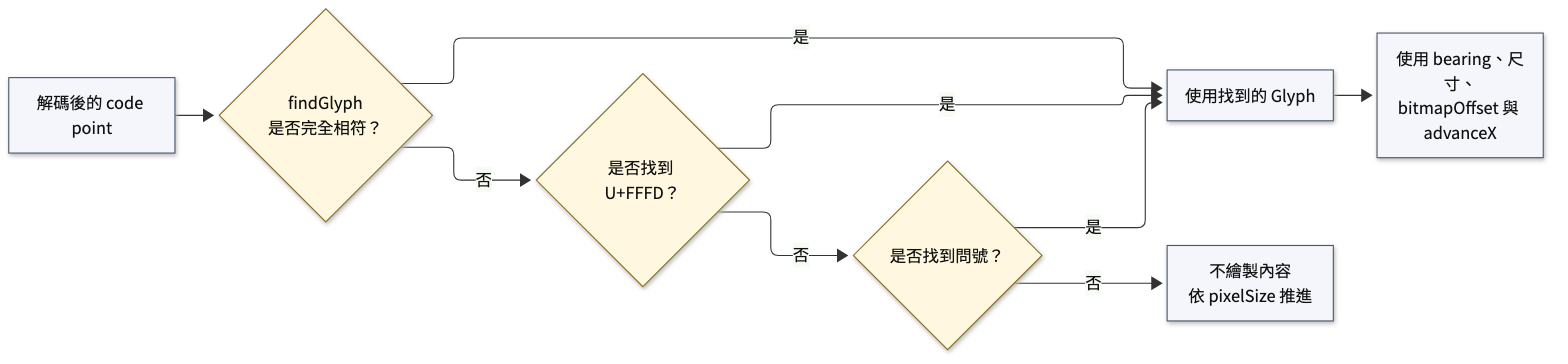
\includegraphics[width=.9\textwidth]{docs/figures/app_b_gfnt-glyph-lookup.png}
    \caption{GFNT Glyph 查找與替代字元使用順序}
    \label{fig:gfnt-glyph-lookup}
\end{figure}

\subsection{Bitmap Rendering}

TextRenderer 以 header 的 ascender/descender 計算 baseline 與 line height。每個 glyph 的左上角為

\[
    x=\text{penX}+b_x, \qquad
    y=\text{baselineY}-b_y.
\]

其中 $b_x$ 與 $b_y$ 是 Glyph 的 horizontal bearing 與 vertical bearing。Bitmap Data 每個 pixel 儲存 alpha；Renderer 讀取目前的 OpenGL color，組成 RGBA pixels，再開啟一般 alpha blending。因為 Glyph rows 由上到下儲存，繪製時使用負的 Y pixel zoom。完成一個 Glyph 後，penX 再增加 \lstinline|advanceX|。整個執行流程已在圖~\ref{fig:gfnt-runtime} 表示。

圖~\ref{fig:gfnt-bitmap-render} 使用實際的 Cubic-11 與 Unifont 字型繪製「你」（U+4F60）。Cubic-11 雖然名稱包含 11，但本專案轉換時使用的 \lstinline|pixelSize| 為 12，因此產生的「你」字 bitmap 為 $13\times11$ pixels，高度是 11 pixels。左半部依 Converter 產生 GFNT 欄位的方式，標出基線、bearing、bitmap 範圍與 advance；右半部則將 Unifont 的 $16\times16$ alpha bitmap 逐格畫出，並顯示 Renderer 如何把目前顏色乘上 Glyph alpha 形成 RGBA pixels。圖中的第一列對應 GFNT Bitmap Data 的起始位置，負的 Y pixel zoom 會讓 \lstinline|glDrawPixels()| 由 Glyph 上方往下顯示。

\begin{figure}[H]
    \centering
    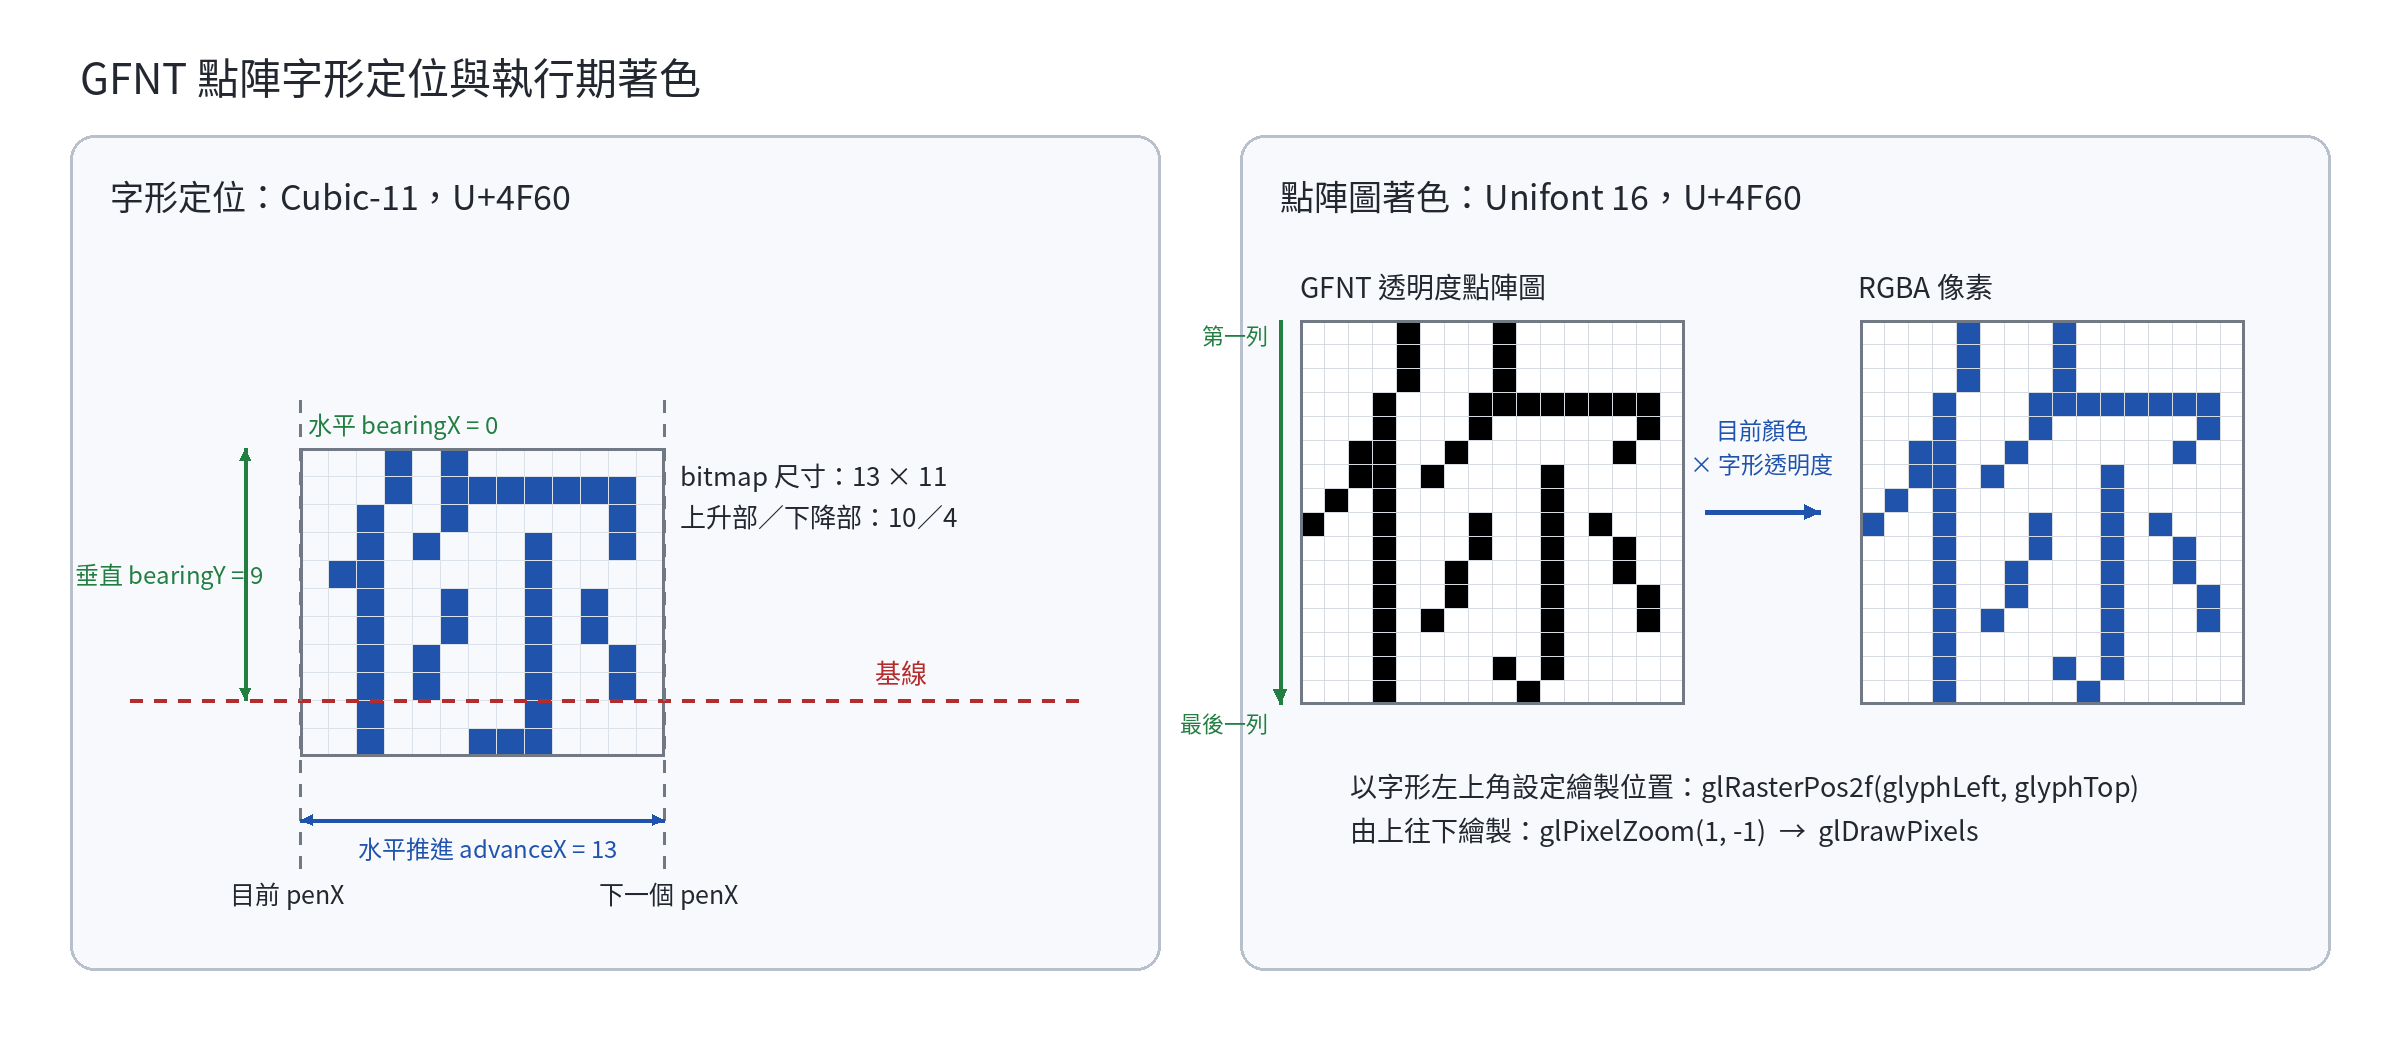
\includegraphics[width=.98\textwidth]{docs/figures/app_b_gfnt-bitmap-render.png}
    \caption{GFNT 字形定位與點陣圖著色；使用 Cubic-11 及 Unifont 16 的實際「你」字點陣圖}
    \label{fig:gfnt-bitmap-render}
\end{figure}
